\documentclass[dvipdfm]{beamer}
\usetheme{Frankfurt}

\usepackage{graphicx}

% XeTeX
\usepackage{fontspec}
\setsansfont{AR PL New Sung}
\XeTeXlinebreaklocale "zh"
\XeTeXlinebreakskip = 0pt plus 1pt
\begin{document}

\begin{frame}
\frametitle{問題描述}
\begin{itemize}
  \item 問題:Failure Candidate Identification for Silicon Debug
  \item 給予以下三個input 檔案:\\
    \begin{enumerate}
      \item verilog 的 pre-silicon flatten gate-level netlist。
      \item silicon simulation 所有 signal 的dump value。
      \item silicon testing 最後所得到的 output value。
    \end{enumerate}
    如果 simulation 跟 testing 所得到的結果為不同的,我們就要做 debug,
    找出所有可能的 defective signal。
\end{itemize}
\end{frame}

\begin{frame}
\frametitle{演算法(Static)}
\begin{itemize}
  \item Static Analysis\\
    \begin{tabular}{|c|c|c|c|c|c|c|}
      \hline
      p & q & and & nand & or & nor & xor\\
      \hline
      0 & 0 & 0   & 1    & 0  & 1   & 0\\
      \hline
      1 & 0 & 0   & 1    & 1  & 0   & 1\\
      \hline
      0 & 1 & 0   & 1    & 1  & 0   & 1\\
      \hline
      1 & 1 & 1   & 0    & 1  & 0   & 0\\
      \hline
    \end{tabular}
  \item 以 and gate 為例,我們將其 input 為 0 的元件放入 candidates 裡面,
    並且只對此元件繼續往下進行 travere,其他 input 則不予理會。
\end{itemize}
\end{frame}

\begin{frame}
\frametitle{演算法(Dynamic)}
\begin{itemize}
\item Dynamic Analysis\\
  \begin{itemize}
    \item 如果已知元件不是 defective signal,
      便從 candidates 刪除僅與此元件連接的 input node。
    \item 因為只有與目前的元件連線,所以可以確定刪除之後,
      不會對尚未作 what-if 的元件造成影響。
  \end{itemize}
\end{itemize}
\end{frame}

\begin{frame}
\frametitle{執行結果}
\begin{itemize}
  \item 使用主辦單位提供之測試資料
  \item 資源的使用量用 GNU time 測量\\
    \begin{tabular}{|l|l|l|l|}
      \hline
             & Case 1 & Case 2 & Case 3\\
      \hline
      \multicolumn{4}{|c|}{元件數量}\\
      \hline
      input   & 4      & 5      & 7\\
      \hline
      output  & 3      & 2      & 3\\
      \hline
      wire    & 4      & 4      & 9\\
      \hline
      gate    & 7      & 6      & 12\\
      \hline
      \multicolumn{4}{|c|}{執行結果}\\
      \hline
      what-if & 3      & 3      & 7\\
      \hline
      final   & 2      & 3      & 6\\
      \hline
      time    & 0 sec  & 0 sec  & 0 sec\\
      \hline
      memory  & 0 KB   & 0 KB   & 0 KB\\
      \hline
    \end{tabular}
\end{itemize}
\end{frame}

\begin{frame}
\frametitle{討論}
\begin{itemize}
  \item 目前 static analysis 相當保守,取得的 candidate 可能不會影響到所有 output%
  \item 如果是用取交集的方式,可以取得最小的 candidate set,但 static analysis 時間會增加
  \item 從經過最多 gate 的 output 開始進行,可以獲得較小的 candidate set,同時能夠減少分析時間
\end{itemize}
\centerline{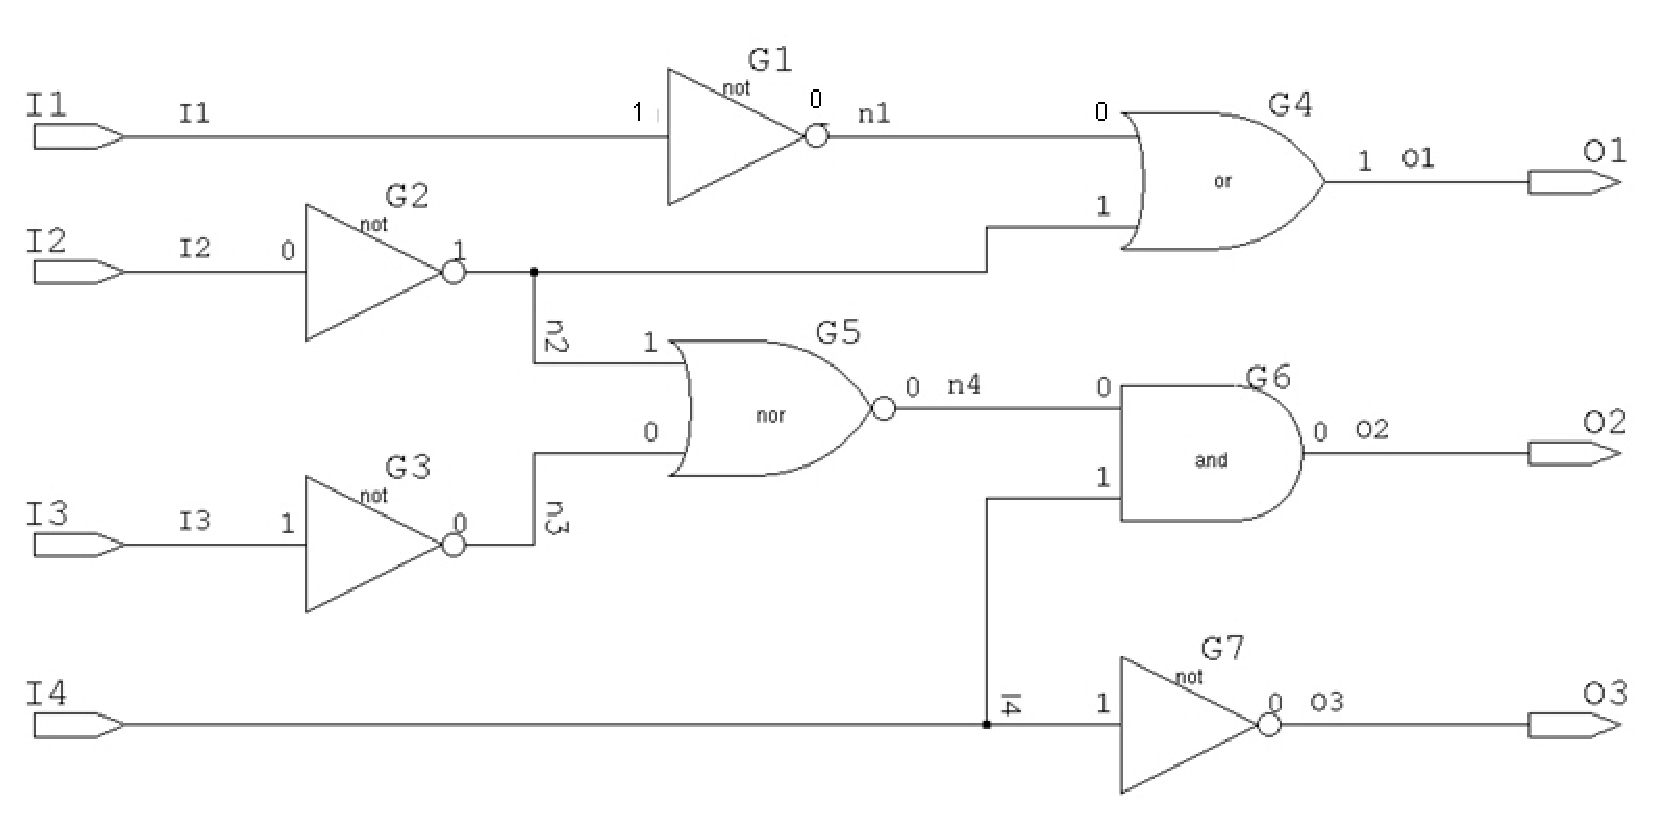
\includegraphics[scale=0.3]{imgs/04.eps}}
\end{frame}

\end{document}
